\chapter[Proposta]{Proposta}
O objetivo deste capítulo é apresentar uma possível proposta de solução, a qual deve atender às necessidades colocadas no primeiro capítulo referente à problemática deste trabalho. A apresentação da proposta está concentrada em duas partes. A primeira parte está relacionada à coleta das métricas utilizando a ferramenta SonarQube, e a segunda parte está relacionada à criação do \textit{dashboard} e à visualização das informações. Para analise da presente proposta, foram escolhidos dois projetos, sendo ambos os projetos de código aberto extraídos do portal do software público brasileiro. A terceira e última parte do trabalho consiste em analisar os resultados obtidos através de uma avaliação qualitativa com possíveis usuários.

\section{Ambiente Simulado}
Para se simular um ambiente de produção, será utilizado como modelo de referência o ambiente apresentado por Luiza e Yago \cite{luiza_yago}. No trabalho descrito, os autores caracterizam o Órgão pertencente à APF como Órgão X. Uma das características referentes ao Órgão X que podem ser citadas diz respeito a sua área de jurisdição que abrange serviços de radiodifusão, postais e de telecomunicações. O Órgão X atualmente implanta o GeDDAS (Gestão de Demandas de Desenvolvimento Ágil de Software) proposto por Souza \cite{souza_sobrinho_uso_2014}. A Figura \ref{img:proc_des} apresenta o processo de desenvolvimento adotado pelo Órgão X.

\graphicspath{{figuras/}}
\begin{figure}[h!]
\centering
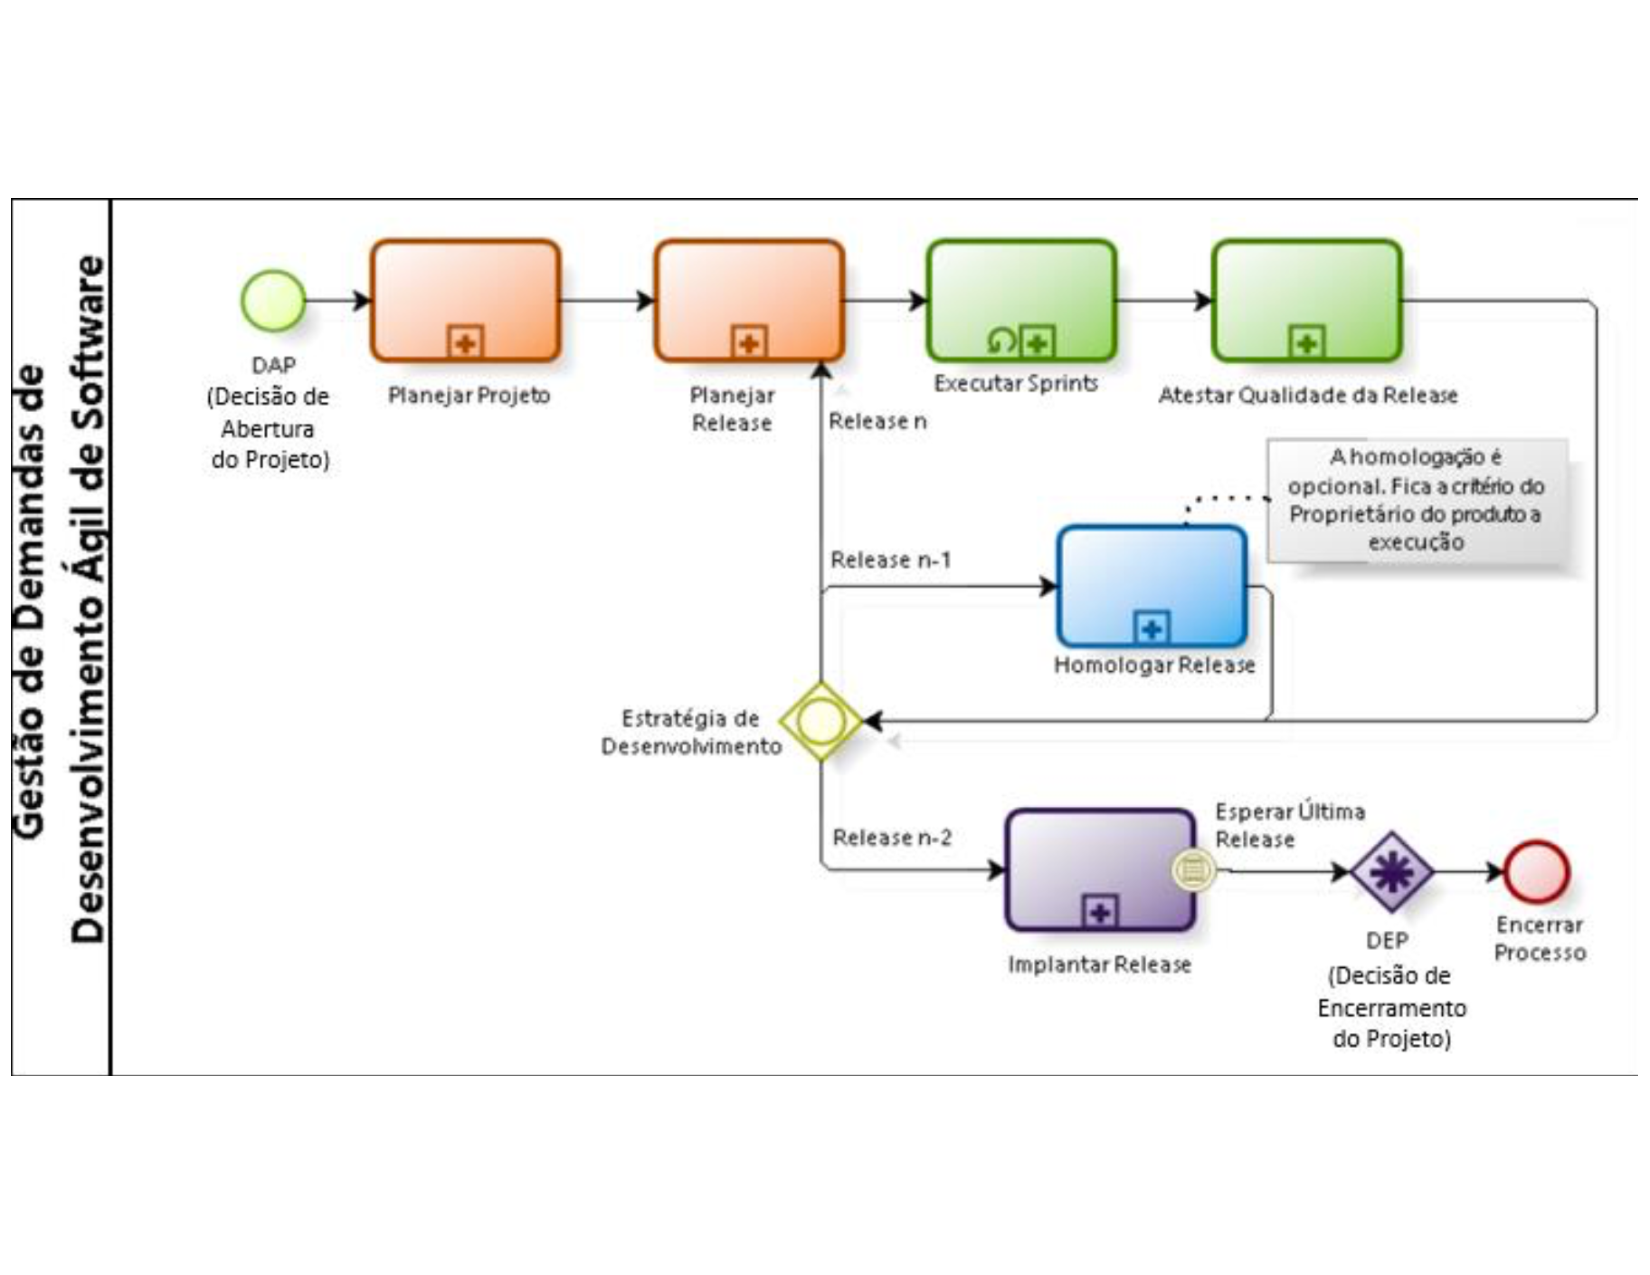
\includegraphics[scale=0.60]{Proc_des.pdf}
\caption{Processo de Desenvolvimento Adotado Pelo Órgão X. Fonte: \cite{luiza_yago}}
\label{img:proc_des}
\end{figure}

A solução proposta tem o objetivo de atuar tanto do lado do Órgão Público, onde o Gestor acompanha o desenvolvimento do projeto, quanto da empresa contratada em que a ferramenta é integrada ao processo de desenvolvimento do software. A Figura \ref{img:ciclo_ver} apresenta um diagrama que demonstra o ciclo de verificação juntamente com a solução apresentada. Na Figura é possível ver que o time de desenvolvimento da empresa contratada desenvolve o código que é submetido para uma análise, onde é feita a verificação das métricas que foram estipuladas. Após essa análise o resultado é submetido para o \textit{dashboard},  o Gestor de TI e a equipe de qualidade do Órgão, podem acompanhar o projeto. A figura \ref{img:diagram_implantacao} apresenta outra visão da integração entre a proposta e o ambiente de configuração do Órgão X.

\graphicspath{{figuras/}}
\begin{figure}[!]
\centering
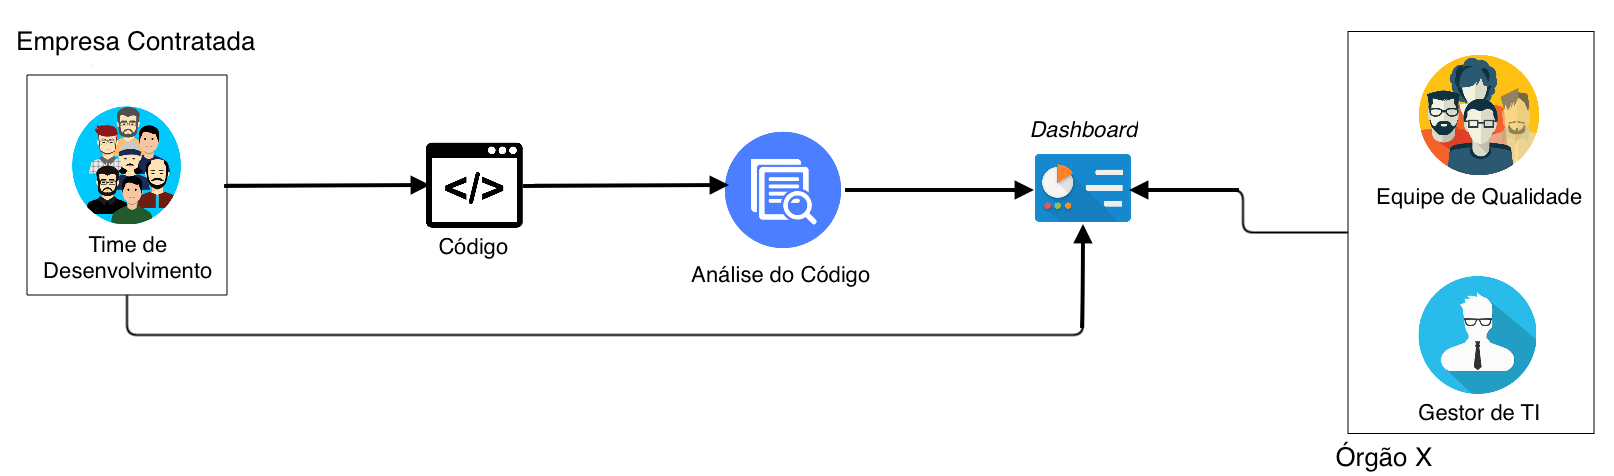
\includegraphics[scale=0.30]{proc_ver.png}
\caption{Ciclo de Verificação Utilizando a Solução Compartilhada Entre Órgão Contratante e Empresa Contratada}
\label{img:ciclo_ver}
\end{figure}

\graphicspath{{figuras/}}
\begin{figure}[!]
\centering
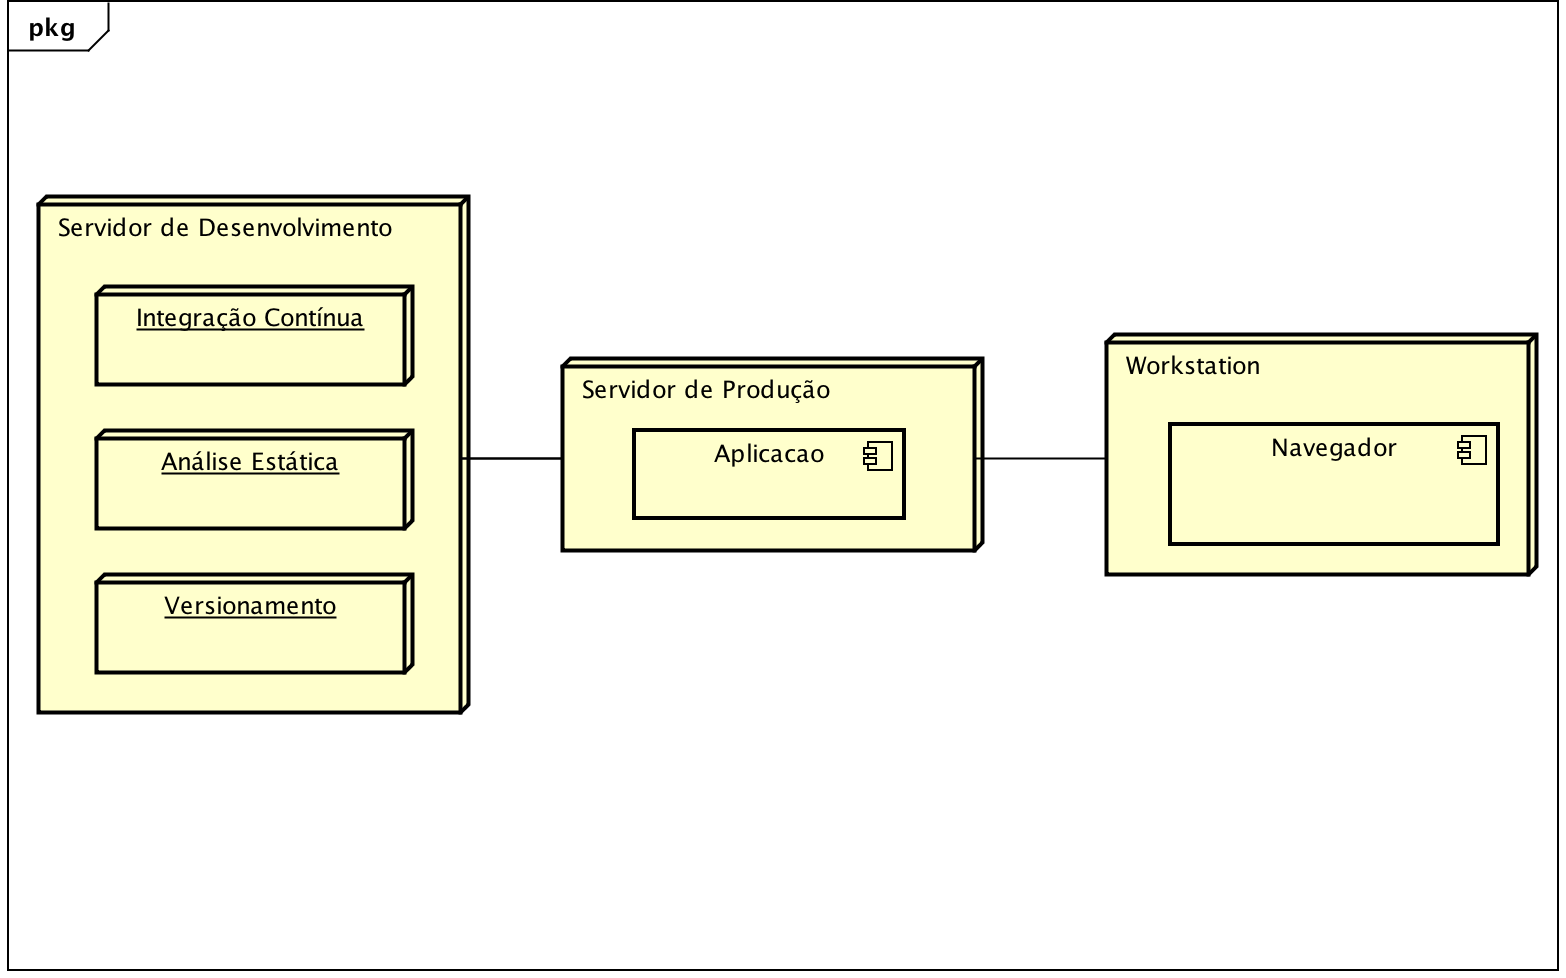
\includegraphics[scale=0.60]{diagrama_implantacao}
\caption{Diagrama de Implantação da Solução no Órgão X} 
\label{img:diagram_implantacao}
\end{figure}



\section{Coleta das Métricas}
Para fazer a coleta das métricas, será utilizada a ferramenta SonarQube. Como já informado na capítulo de Suporte Tecnológico, esse suporte é muito utilizado em Órgãos Públicos e em editais por ser uma ferramenta \textit{open-source}. Nesse contexto, a coleta das métricas é feita de maneira dinâmica, onde o que usuário decide qual suíte de métricas vai utilizar, podendo utilizar uma customizada ou utilizar uma como base. A presente proposta irá utilizar as suítes de métricas estabelecidas no edital do DNPM \cite{edital}). Portanto, serão utilizadas as suítes de métricas de Chidamber-Kemerer e a Suíte MOOD.

Essas métricas serão atribuídas ao longo do desenvolvimento do projeto, sendo assim, durante as primeiras \textit{sprints} do projeto serão utilizadas métricas diferentes e mais relevantes ao andamento do projeto, dos que as métricas que serão coletadas ao fim do projeto. A escolha das métricas a serem utilizadas em cada momento do desenvolvimento será feita através de um questionário com até quatro gerentes de projeto e uma persona criada para simular um gestor "ideal".

As métricas "Violações do tipo Blocker", "Violações do tipo Major" e "Violações do tipo Minor" são estipuladas de acordo com o próprio perfil do Sonar, chamado Sonar Way. Contudo, a melhor maneira seria criar um perfil com as regras da própria organização garantindo uma avaliação mais focada no objetivo do Órgão.


O objetivo deste trabalho é criar uma ferramenta que auxilie na auditoria de produtos de software entregues por empresas terceirizadas. Entretanto percebe-se que ainda que o trabalho possua grande aprovação, dificilmente o mesmo irá substituir o fator humano da auditoria. Portanto, o software compreende apenas um suporte que visa facilitar a avaliação geral do software entregue sob o ponto de vista da qualidade de código. Recomenda-se, uma vez que o software seja submetido à ferramenta e seja aceito, a realização de uma auditoria em cima de uma amostragem do software entregue, sob o olhar de um analista especializado para tal atividade.

Foi elaborado uma prova de conceito, para que se pudesse testar a funcionalidade relacionada à coleta de métricas. Está prova, consiste em, elaborar um software que fosse capaz de extrair métricas do relatório do SonarQube. Inicialmente foi necessário criar uma instância do SonarQube e fazer a análise de um projeto. O projeto escolhido foi um projeto em Java, que o próprio SonarQube disponibiliza para download, com o intuito de ser utilizado como exemplo. Com o ambiente configurado, implementou-se uma solução em Python que atendesse aos requisitos estabelecidos para a prova de conceito. A Figura \ref{img:terminal} apresenta a saída do console, ao se rodar a solução.


\graphicspath{{figuras/}}
\begin{figure}[H]
\centering
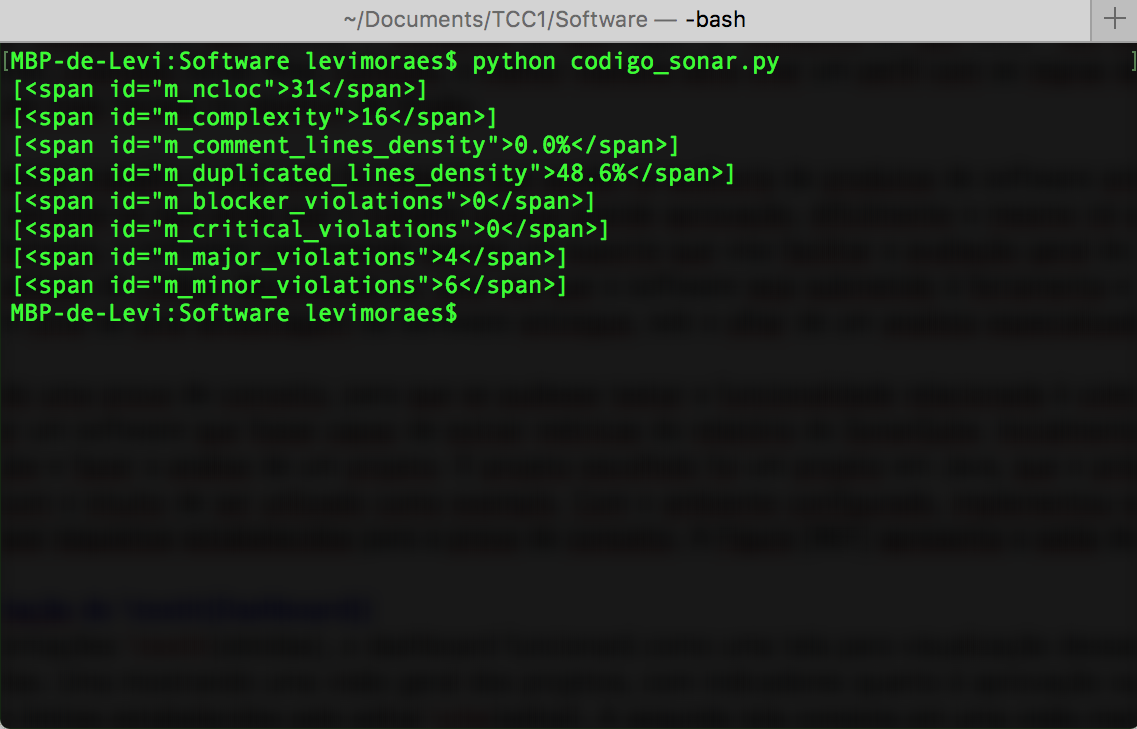
\includegraphics[scale=0.60]{terminal.png}
\caption{Métricas Extraídas do SonarQube}
\label{img:terminal}
\end{figure}

Na primeira linha da Figura \ref{img:terminal}, é executada a chamada do código. As linhas seguintes apresentam as métricas coletadas pela solução. As métricas que são apresentadas no console, foram definidas no código, por este motivo, ainda não é possível definir outras métricas durante a execução da aplicação, esta funcionalidade será implementada na segunda fase do projeto. 

\section{Criação do \textit{Dashboard}}
Com as informações obtidas, o dashboard funcionará como uma tela para visualização dessas métricas. A solução é composta por duas telas. Uma mostrando uma visão geral dos projetos, com indicadores quanto à aprovação ou reprovação de cada projeto seguindo os limites estabelecidos pelo edital \cite{edital}. A segunda tela consiste em uma visão mais detalhada sobre cada projeto, mostrando a evolução do projeto em cada métrica e com um \textit{link} para o Sonar de cada métrica para um aprofundamento.

Para melhor compreensão da proposta, foram elaborados protótipos das possíveis telas que farão parte da solução final. A Figura \ref{img:telaLogin} apresenta a tela inicial da solução, por onde o Gestor fará o acesso colocando seu \textit{username} e seu \textit{password}. Ainda nesta tela, existe um \textit{link} para caso o Gestor não se lembre do seu \textit{password}, onde o sistema enviará uma mensagem, para o \textit{email} cadastrado, solicitando a alteração.

\graphicspath{{figuras/}}
\begin{figure}
\centering
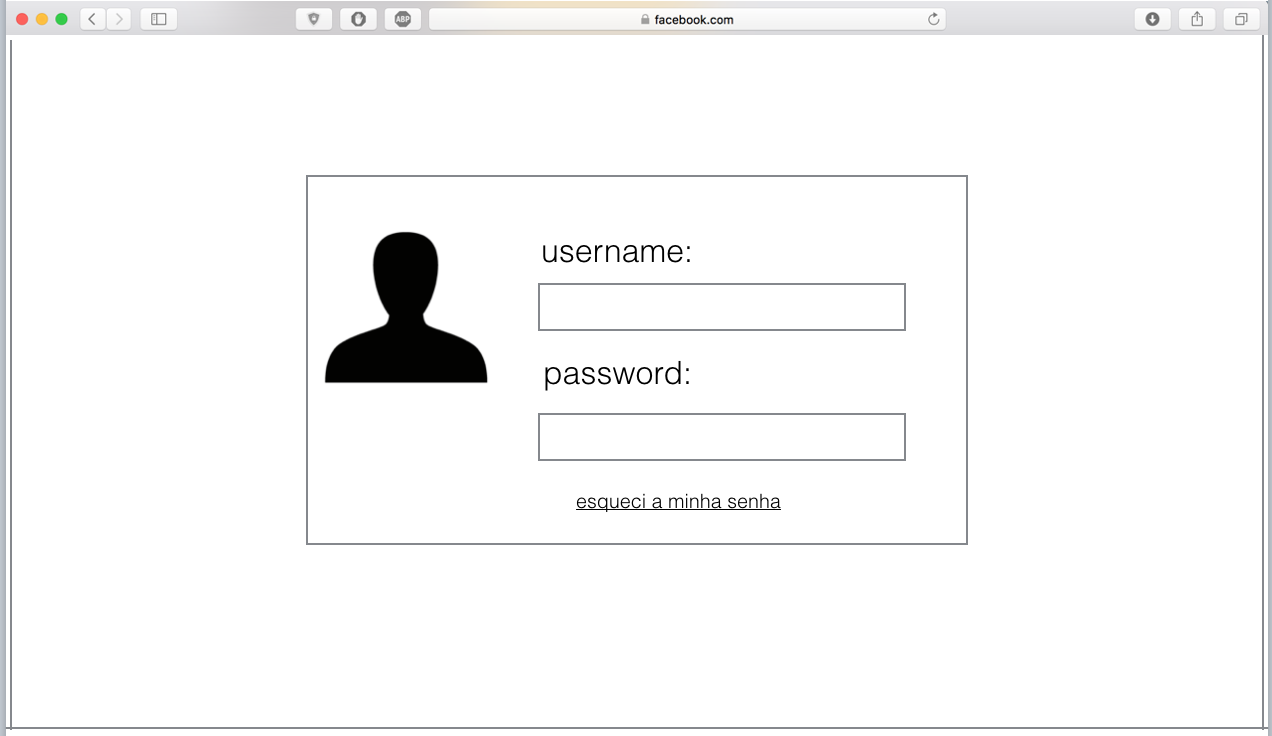
\includegraphics[scale=0.60]{telaLogin.png}
\caption{Tela Login}
\label{img:telaLogin}
\end{figure}

A página inicial da solução, também chamada de \textit{home page}, aqui apresentada na Figura \ref{img:telaHome}. Nesta página, o Gestor tem uma visão de todos os projetos, que ele cadastrou para serem acompanhados. Cada projeto é representado por um retângulo de uma cor , e neste retângulo estão algumas informações referentes ao projeto, que podem ser visualizadas, sem a necessidade de se abrir o projeto. Tanto as cores dos retângulos, como as informações dos projetos podem ser customizadas de acordo com o Gestor. Nesta página, ainda existe um botão que direciona o usuário para a tela de "adicionar projetos". Esta tela é somente para o gestor.
 
\graphicspath{{figuras/}}
\begin{figure}
\centering
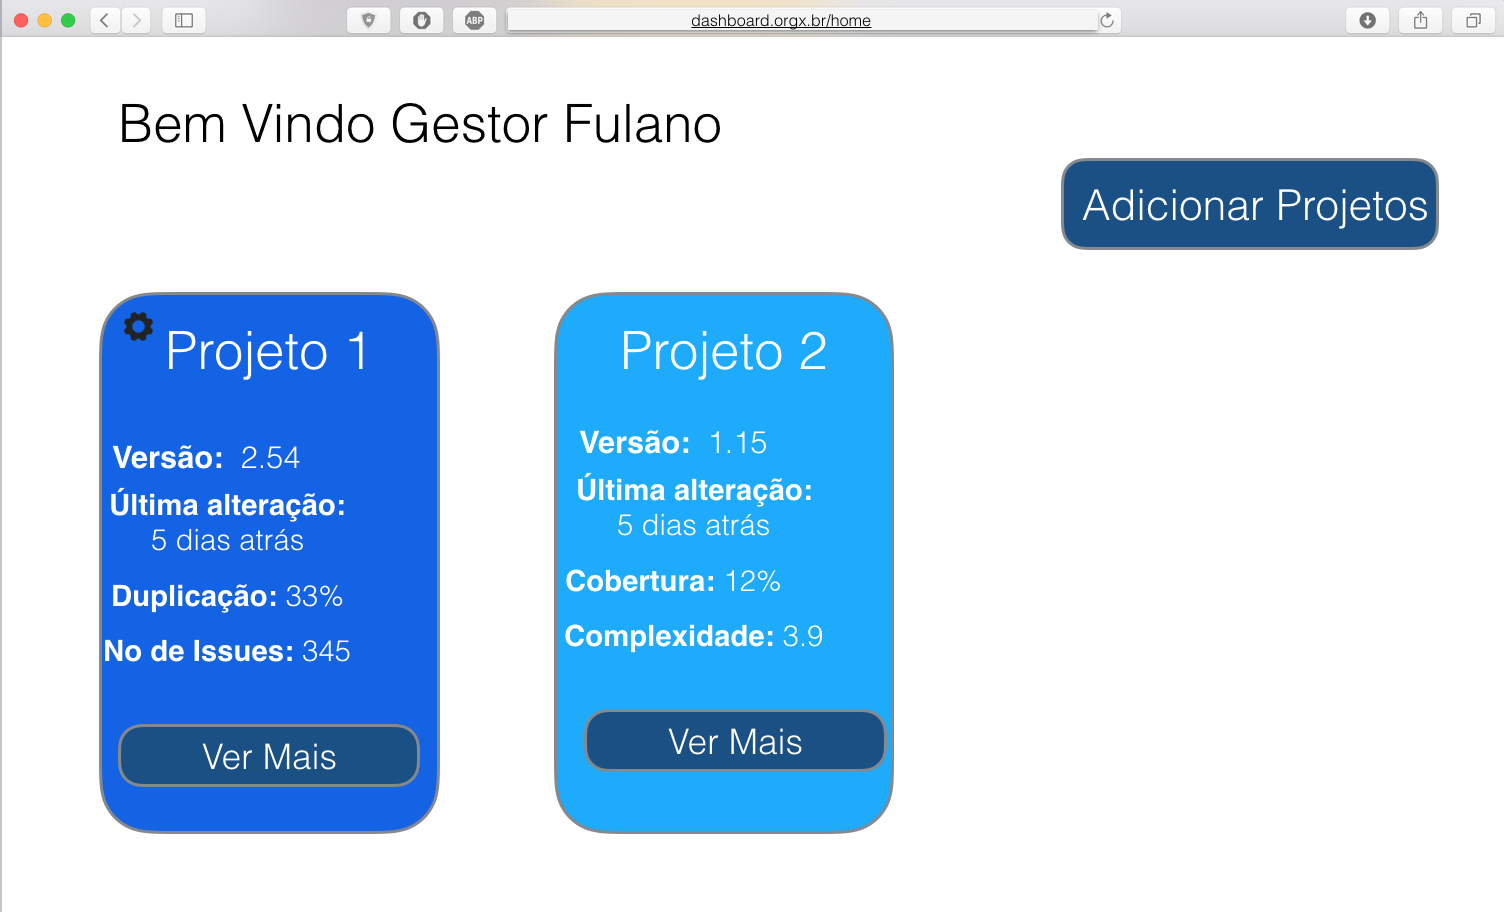
\includegraphics[scale=0.60]{telaHome2.png}
\caption{Tela Home}
\label{img:telaHome}
\end{figure} 

A Figura \ref{img:telaDashboard} apresenta um protótipo do \textit{dashboard} que será implementado. Nesta página encontram-se as informações referentes ao projeto selecionado. Está página apresenta em forma de gráficos, as métricas que foram selecionadas pelo Gestor para aquele projeto. Esta é a única página que pode ser acessada pela empresa terceirizada. Em cada métrica é possível passar a seta seletora por cima do ícone "?" para que se tenha uma breve explicação da métrica 

\graphicspath{{figuras/}}
\begin{figure}
\centering
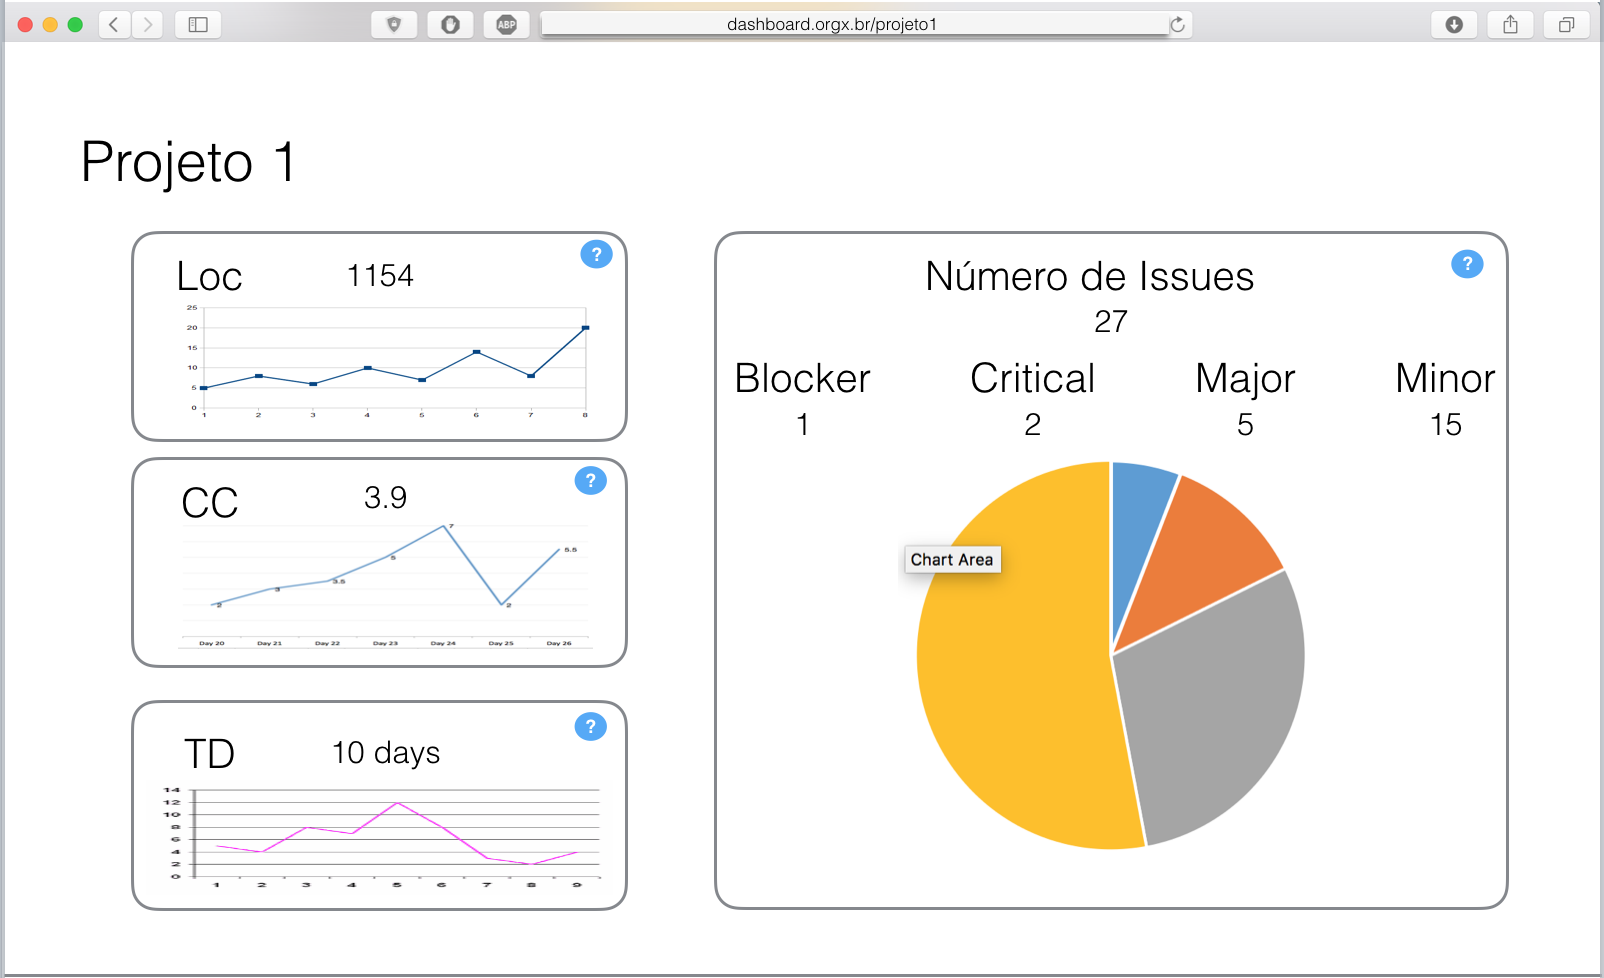
\includegraphics[scale=0.60]{telaDashboard.png}
\caption{Tela Dashboard}
\label{img:telaDashboard}
\end{figure} 

Para se fazer a adição de um novo projeto, é necessário que o projeto a ser adicionado, esteja armazenado em um repositório que o Gestor tenha acesso de leitura. A Figura \ref{img:telaAdicionar} representa um protótipo da página de adição de projetos. Nesta página são adicionados, o nome do projeto, uma descrição, a url do repositório em que se encontra o projeto e por último, as métricas que serão analisadas. Assim como na página do \textit{dashboard}, cada métrica apresenta um ícone "?" que apresenta uma breve explicação de cada métrica.

\graphicspath{{figuras/}}
\begin{figure}
\centering
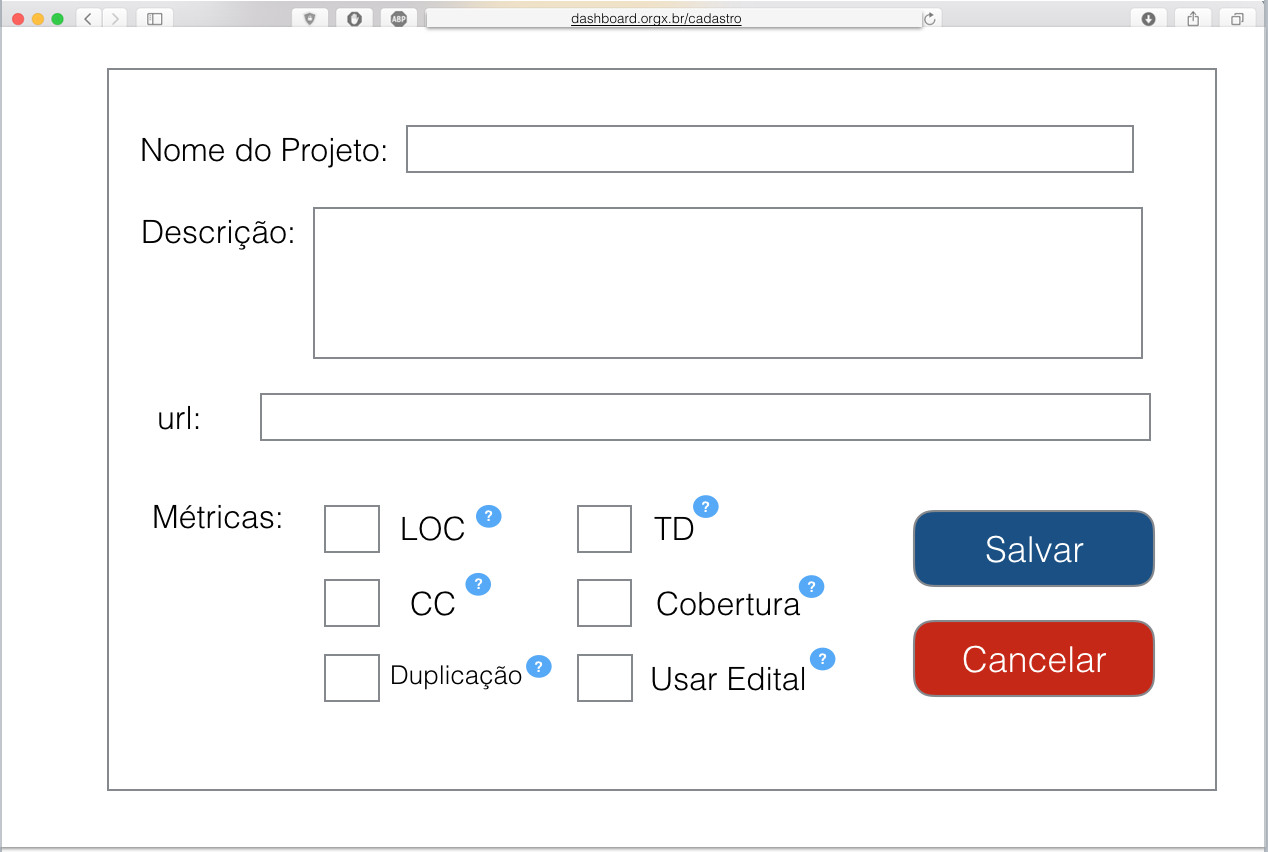
\includegraphics[scale=0.60]{telaAdicionar.png}
\caption{Tela Adicionar}
\label{img:telaAdicionar}
\end{figure} 

Assim como a coleta de métricas, também foi elaborada uma prova de conceito, para testar a exibição dos gráficos que seriam mostrados no \textit{dashboard}. Esta era uma continuação da prova de conceito da coleta de métricas, em que, feita a coleta, deveria-se exibir as métricas em um gráfico. A Figura \ref{img:dashboard} apresenta a tela relacionada à esta prova de conceito.

\graphicspath{{figuras/}}
\begin{figure}[H]
\centering
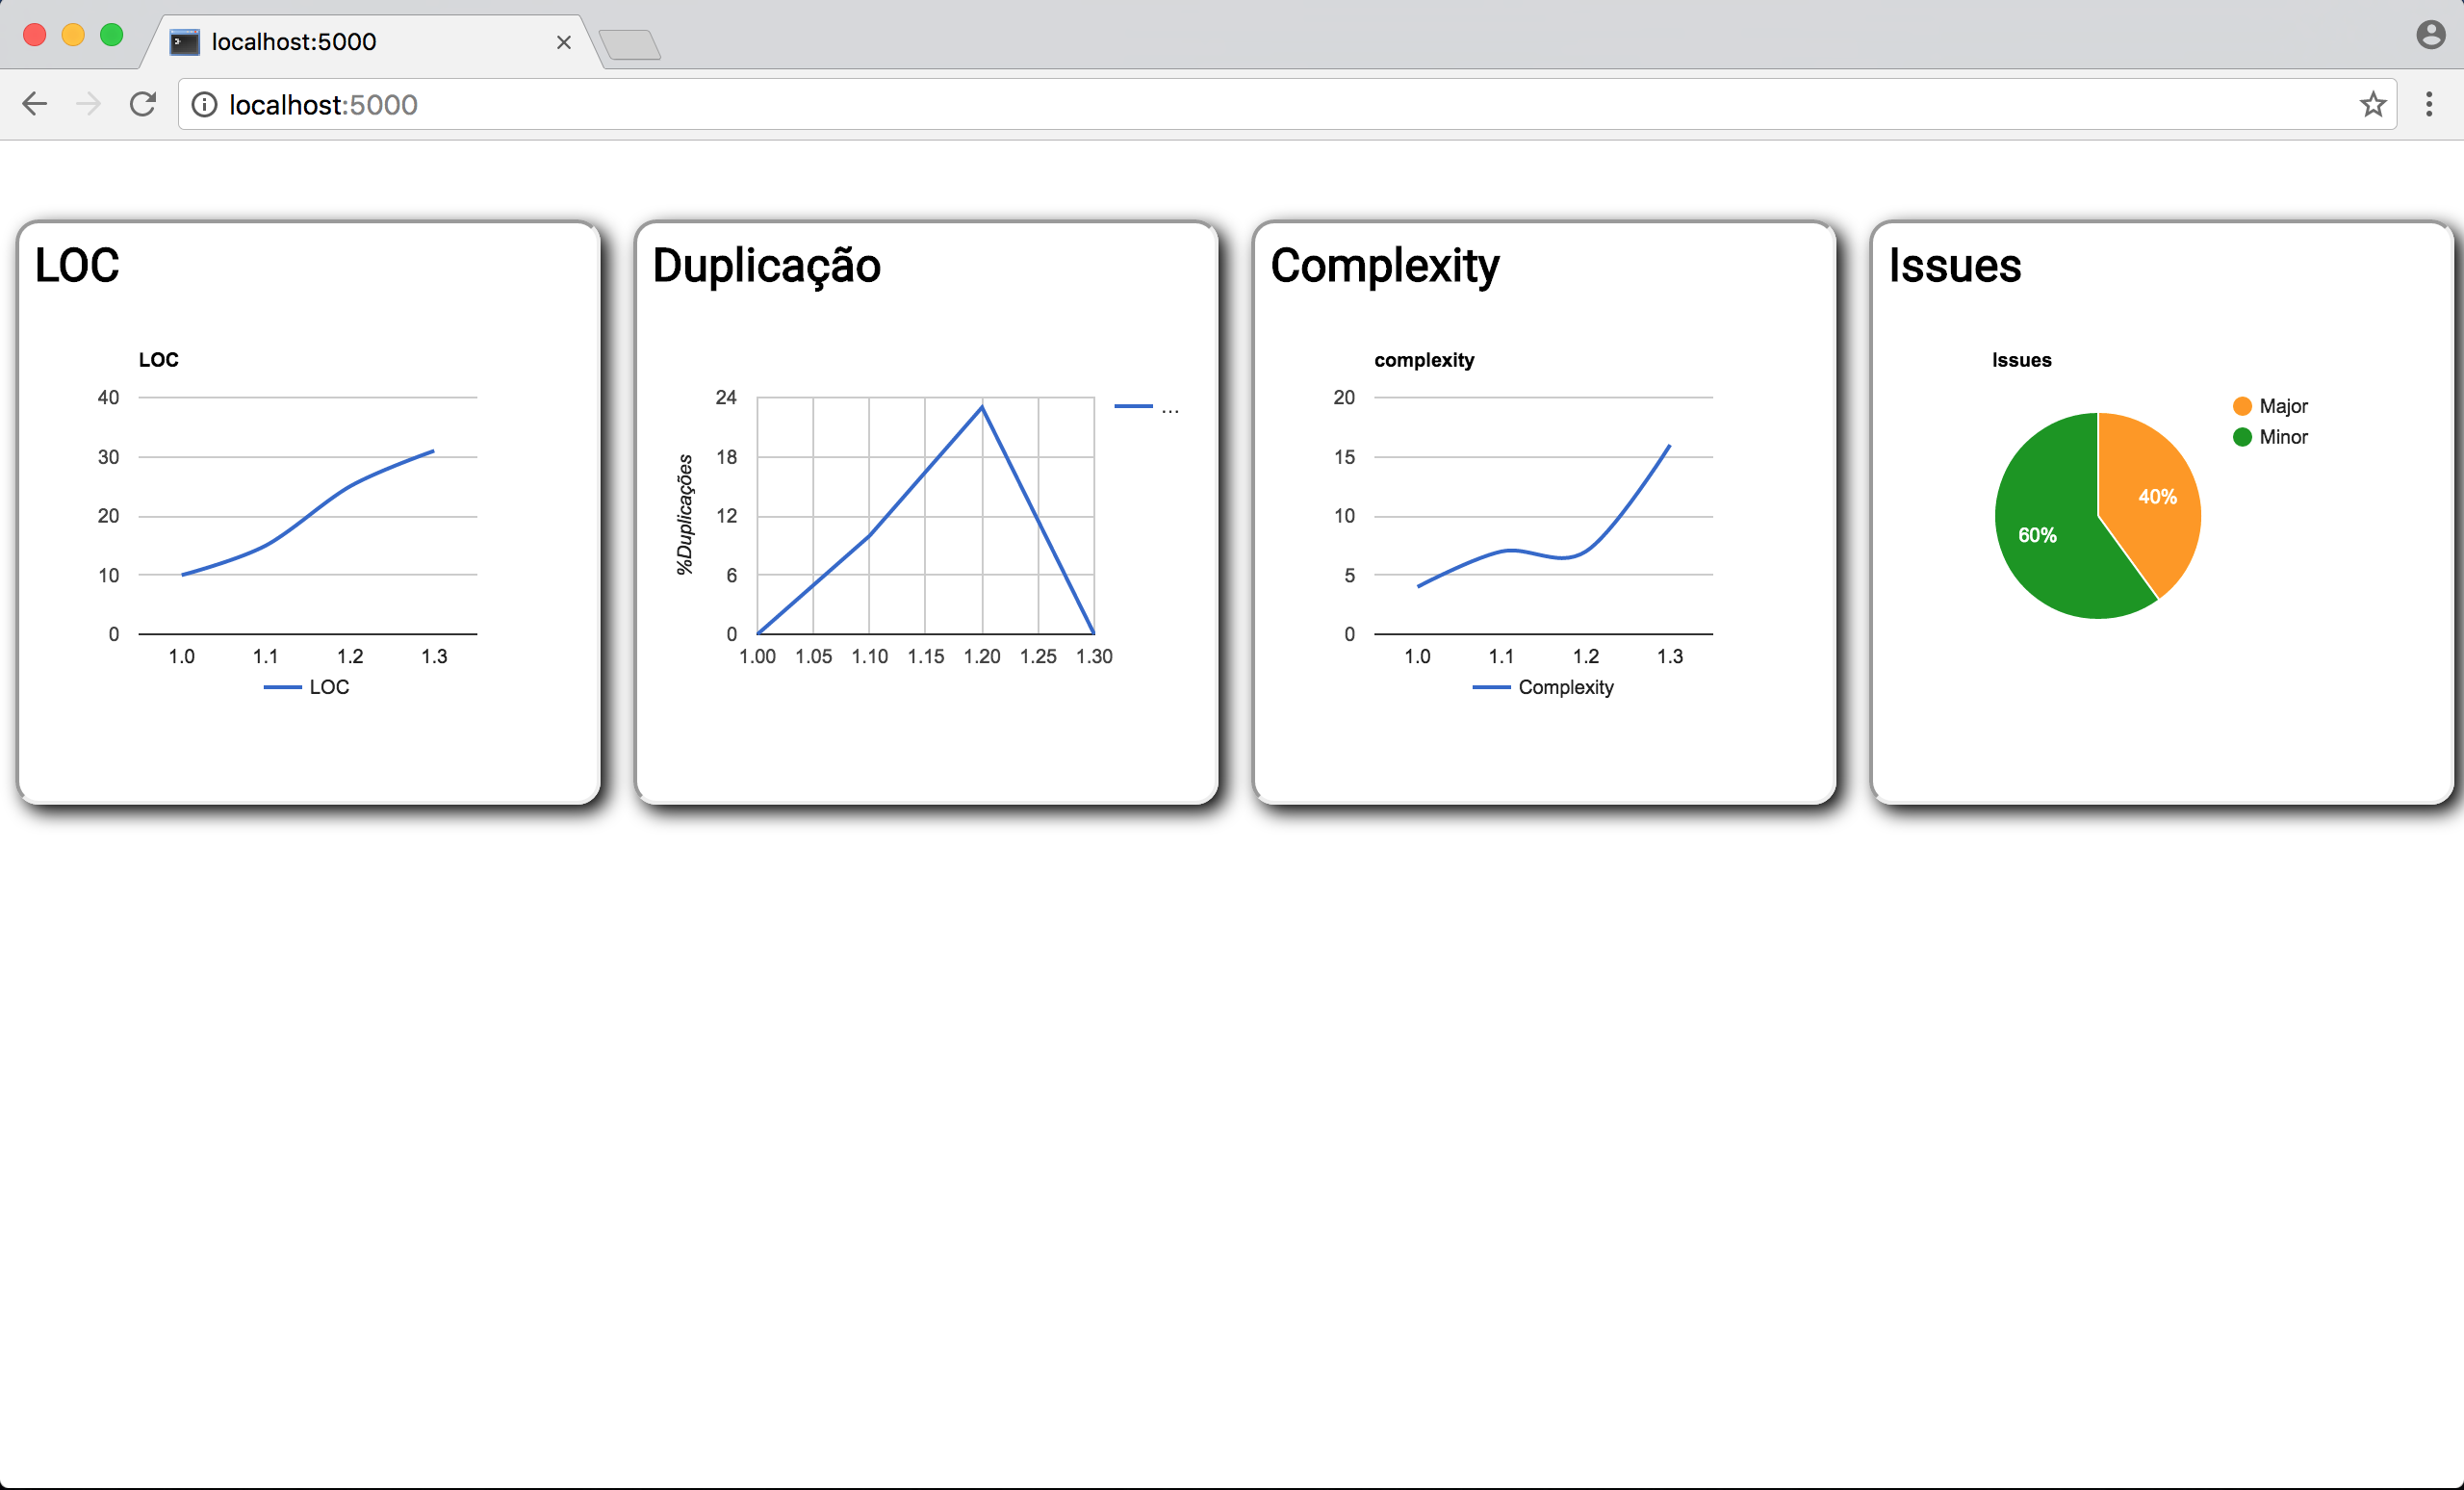
\includegraphics[scale=0.35]{dashboard_conceito.png}
\caption{Página do \textit{Dashboard} da Prova de Conceito}
\label{img:dashboard}
\end{figure}

\section{Avaliação}
A avaliação do \textit{dashboard} será feita por parte de um gestor de tecnologia de um Órgão Público. Ele avaliará aspectos de usabilidade da ferramenta e se a ferramenta possuiria condições mínimas de ser implantada. Caso não seja possível essa avaliação com um profissional da área, a avaliação será feita através de professores que possuem tal experiência com contratação de software para Órgãos Públicos, novamente avaliando aspectos como usabilidade e melhorias necessárias para implantação em um Órgão.
Para fazer esta avaliação, o gestor responderá a um questionário contendo, inicialmente, cinco perguntas, referentes ao uso e às funcionalidades do software produzido. Uma primeira versão do questionário consta na Figura \ref{img:questionario}

Uma segunda parte da avaliação se refere a usabilidade do software desenvolvido. Para fazer esta avaliação será utilizado o modelo de questionário SUS

\section{Resumo do Capítulo}
A proposta deste trabalho é criar uma maneira facilitada de acompanhar a qualidade de código estático dos produtos de software entregues pelas tercerizadas. Para fazer esta análise, a solução orienta-se por uma ferramenta de análise estática SonarQube e por um conjunto de métricas relacionadas às boas práticas de programação, algumas dessas métricas, foram retiradas dos livros Clean Code \cite{martin2009clean} e Code Complete \cite{mcconnell2004code}. A solução encontrada é a utilização de um \textit{dashboard} que mostre o real estado de um projeto, e que através de indicadores, seja possível determinar a qualidade do código. A última etapa deste trabalho consiste na avaliação do trabalho produzido, a qual será feita juntamente com um gestor de projeto de um Órgão Público ou um professor da instituição de ensino que responderá a um questionário quanto ao software produzido.